\section{Diffusion-Reaction Equation With Forced Current through the system.}

We consider the same system as above

\begin{align}
	\frac{\partial C}{\partial t} = \mathcal{D}\frac{\partial^2 C}{\partial x^2},
\end{align}

with a slight change in border conditions. We want to impose the current on the system, which should be proportional to the reaction rate at the interface.

\begin{align}
	R &= k_f C(0^+, t)\\ 
	&= \frac{i_0}{\mathcal{F}}.
\end{align}

This yields the following border and initial conditions for the problem

\begin{align}
	C(\delta, t) &= C_b,\\
	C(0^+, t) &= \frac{R}{k_f},\\
	C(x, 0) &= 0.
\end{align}

or equivalently

\begin{align}
	C(\delta, t) &= C_b,\\
	C(0^+, t) &= \frac{i_0}{\mathcal{F}k_f},\\
	C(x, 0) &= 0.
\end{align}


Appendix \label{appendix:forced-current-analytic} shows the procedure to calculate the analytic solution. The particular solution to the system is




\begin{align}
	C(x, t) = \frac{i_0}{\mathcal{F}k_f} +\qty{C_b - \frac{i_0}{\mathcal{F}k_f}}\frac{x}{\delta} +\frac{2}{\pi}\sum_n \qty{(-1)^n C_b- \frac{i_0}{k_f\mathcal{F}}} \frac{\exp{\left[-n^2\pi^2\frac{\mathcal{D} t}{\delta^2}\right]}}{n}\sin\left(n\pi\frac{x}{\delta}\right).
\end{align}



\newpage


The numerical algorithm is outlined in detail in Appendix \ref{appendix:numeric-solution-forced}. \ref{fig:forced-current-dynamic}.

\begin{figure}[htbp]
\centering
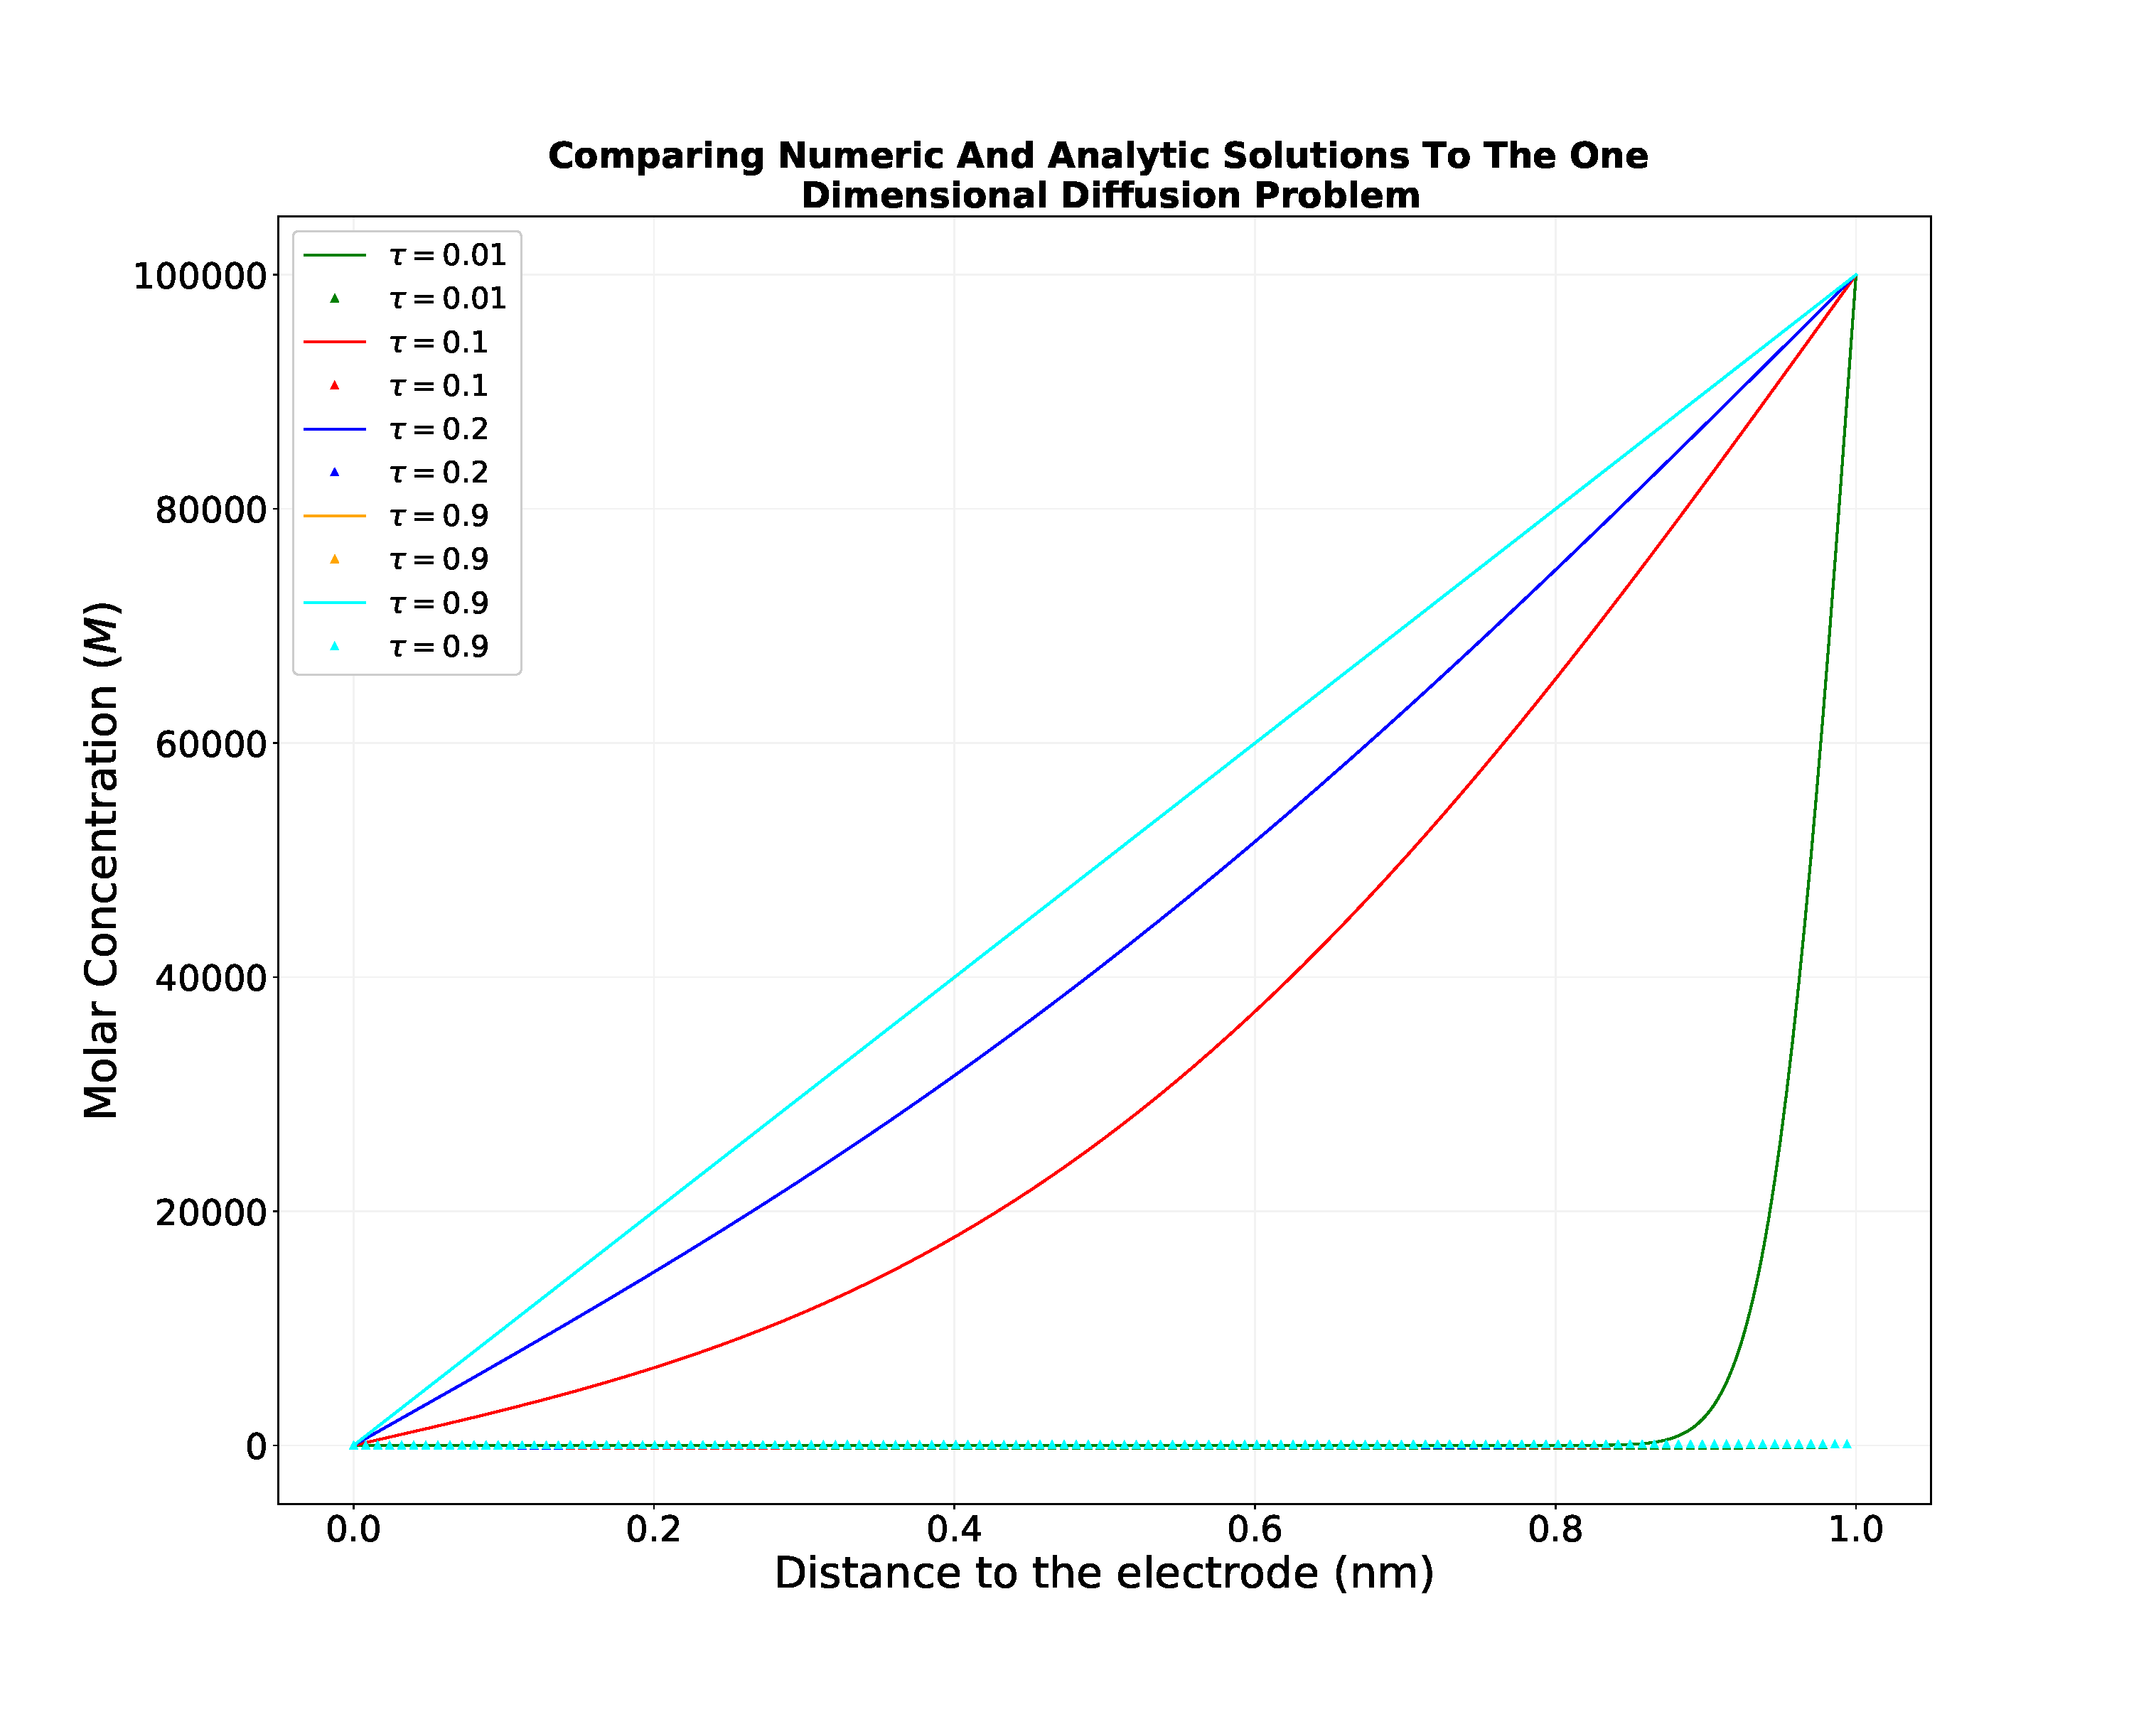
\includegraphics[width=\textwidth]{forced-current-dynamic.eps}
\caption{Comparison between numerical an analytical results. The numerical method  (dotted line) behaves as expected, following the analytical solution.}
\label{fig:forced-current-dynamic}
\end{figure}
